% --------------------------------------------------------------------

\section{Johdanto}

Ohjelmistoprojekteissa tulee väistämättä vastaan ongelmia. Näiden järjestelmällinen analysointi ja ehkäiseminen jatkuvana osana kehitysprosessia parantaa ohjelmistoprojektin mahdollisuuksia onnistua. Ketterässä ohjelmistokehityksessä kehitystiimi järjestää säännöllisesti reflektion, jossa tiimi tarkastelee työtapojaan ja tiimityöskentelyään, sekä pohtii tapoja, joilla voi sopeuttaa niitä päästäkseen parempiin tuloksiin \citep{AgileRetros2006}. Retrospektiivissä kehitystiimi pyrkii tutkimaan konkreettisia ongelmia ja löytämään niihin konkreettisia ratkaisuja \citep{AgileRetros2006}. Juurisyyanalyysi (RCA, Root Cause Analysis) tarjoaa rakenteellisen tavan löytää ongelmien aiheuttajia ja voi siten auttaa ehkäisemään näiden ongelmien esiintymistä jatkossa \citep{Lehtinen2011}. Rakenteellinen tapa tunnistaa ongelmien aiheuttajia sopii hyvin retrospektiivin ongelmanratkaisuun \citep{Lehtinen2013}. Juurisyyanalyysiä voi kuitenkin tehdä lukuisalla eri tavalla \citep{Lehtinen2011}.

Vaikka iteraation lopussa pidettävä retrospektiivi on olennainen osa ketterän ohjelmistokehitysprosessin runkoa, ei sen toteutustapavasta ole yhteistä käytäntöä. Iteraatiolla tarkoitetaan ketterissä ohjelmistokehitysmenetelmissä suosittuja lyhyitä kehityssyklejä, joihin ohjelmointityö on jaettu \citep{beck1999embracing}. Iteraation voi mieltää pieneksi, enintään kuukauden pituiseksi projektiksi \citep{ScrumGuide2011}. Retrospektiivin järjestäminen on määritelty ketterien menetelmien yleisissä periaatteissa \citep{AgileManifestoPrinciples}. Retrospektiivin tavoitteet saattavat olla määritelty tarkasti kunkin ketterän ohjelmistokehitysmetodologian kuvauksessa, mutta sen toteutustapa on usein jätetty tiimin päätettäväksi. Esimerkiksi Scrum-metodologian kuvauksessa on kuvattu retrospektiivien tavoitteet, muttei niiden saavuttamiseen johtavia menetelmiä \citep{ScrumGuide2011}.

Tässä kandidaatintyössä tutkitaan systemaattisen kirjallisuuskatsauksen \citep{Kitchenham2010} avulla juurisyyanalyysiä soveltavia retrospektiivejä. Työssä vastataan seuraaviin tutkimuskysymyksiin:
\begin{enumerate}
\item Minkälaisia menetelmiä aiemmassa kirjallisuudessa on esitetty juurisyyanalyysiä soveltaviin retrospektiiveihin?
\item Minkälainen menetelmä voisi sopia ketterän ohjelmistokehitystiimin retrospektiiviin?
\end{enumerate}
Menetelmän tulee olla kevyt ja yksinkertainen toteuttaa, jotta sen käyttöönotto lyhyehköissä iteraatio-retrospektiiveissä olisi mielekästä. Esimerkiksi extreme programming -metodologiaan on suositeltu lyhyitä ja tehokkaita retrospektiivejä, jotka eivät vaadi kovin suurta panosta tiimiltä, mutta tuottavat siitä huolimatta välittömiä ja näkyviä tuloksia \citep{myllyaho2004review}. Systemaattisen kirjallisuuskatsauksen aineistohaut rajoitettaan Scopus-tietokannan tieteellisiin artikkeleihin.

Tämä kandidaatintyö on jaettu seuraaviin osiin. Kappaleessa 2 esitellään teoreettinen tausta, joka sisältää määritelmät ketterälle retrospektiiville ja juurisyyanalyysille. Kappaleessa 3 kuvataan työssä käytetyt tutkimusmenetelmät. Kappaleessa 4 tuodaan julki tulokset ja kappaleessa 5 tulosten johtopäätökset ja kandidaatintyln tuloksiin liittyvät validiteettiuhat. Kandidaatintyön viimeinen kappale on yhteenveto.

\section{Teoreettinen tausta}

\subsection{Ketterä retrospektiivi}
Ketterissä ohjelmistokehitysmenetelmissä on määritelty, että säännöllisin väliajoin pidetään reflektointi, jossa kehitystiimi pohtii tapoja tulla tehokkaammaksi. Kehitettyjen parannusehdotusten perusteella tiimi muuttaa toimintaansa \citep{AgileManifestoPrinciples}. Kevyt retrospektiivisessio on tapa toteuttaa tätä reflektointia \citep{Cockburn2002}. Projektin lopputuloksen kannalta retrospektiivejä on perusteltua pitää lyhyin väliajoin \citep{Cockburn2002}. Tällöin tiimin kohtaamat ongelmat ja niihin liittyvät yksityiskohdat ovat tuoreessa muistissa ja parannusehdotukset voidaan ottaa suoraan käyttöön ja siten pyrkiä parantamaan projektin lopputuloksen laatua \citep{Cockburn2002}.

XP- ja Scrum-metodologiassa retrospektiivejä suositellaan pidettäväksi joka iteraation päätteeksi \citep{Lindstrom2004, ScrumGuide2011}. Iteraatioretrospektiiveissä kehitystiimi reflektoi sitä, missä he ovat viime iteraation aikana onnistuneet hyvin ja missä on vielä kehitettävää \citep{Lindstrom2004, ScrumGuide2011}. Retrospektiivin avulla tiimi saa palautetta työstään \citep{Lindstrom2004}. Retrospektiivissä voidaan muun muassa pohtia sitä, miten kurinalaisesti kehitystiimi on noudattanut työkäytäntöjä ja voisiko niitä räätälöidä sopimaan paremmin tiimin tarpeisiin \citep{Lindstrom2004}.

\subsection{Juurisyyanalyysi}
Juurisyyanalyysi on rakenteellinen tapa tutkia ongelmia ja tunnistaa niiden aiheuttajia \citep{Lehtinen2011}. Juurisyyanalyysi pohjautuu teoriaan, jonka mukaan ongelman uudelleenesiintyminen voidaan välttää kontrolloimalla sen aiheuttajia \citep{Lehtinen2011}. Juurisyyanalyysin avulla voidaan tutkia ongelmien lisäksi myös onnistumisten syitä. \citep{Bjornson2009} Juurisyylle on useita määritelmiä \citep{Lehtinen2011}. Se voi tarkoittaa mitä tahansa ongelman aiheuttavaa syytä, syyketjun perimmäisintä syytä tai syytä, johon johto voi vaikuttaa \citep{Lehtinen2011}. Juurisyyanalyysin tuloksia voidaan käyttää apuna prosessinkehityksessä. \citep{Lehtinen2011}

\section{Systemaattinen kirjallisuuskatsaus tutkimusmenetelmänä}

\subsection{Taustaa}
Systemaattisessa kirjallisuuskatsauksessa (SLR, Systematic Literature Review) tehdään kattava arviointi valitusta aiheesta. Arvioinnissa käytetään luotettavaa, tarkkaa ja toistettavissa olevaa menetelmää. SLR on kirjallisuuskatsauksen muoto, mikä tarkoittaa sitä, että siinä käydään läpi aiempia tutkimuksia, jotka ovat olennaisia työssä esitettävien tutkimuskysymysten kannalta. Kerätyn kirjallisuuden pohjalta muodostetaan synteesi, eli kerätään, yhdistetään ja tehdään yhteenveto kerätystä aineistosta. \citep{Kitchenham2007}

SLR:n erityispiirteenä on se, että kirjallisuuden etsiminen, valikointi ja valitun kirjallisuuden analysointi pyritään tekemään toistettavasti ja objektiivisesti. Kitchenham perustelee SLR-menetelmän hyötyä toteamalla, että kirjallisuuskatsaus, joka ei ole SLR:n tapaan perusteellinen ja tasapuolinen, ei tarjoa paljoa tieteellistä arvoa. Systemaattisen kirjallisuuskatsauksen tulokset ovat todennäköisemmin objektiivisia, eli tutkijan kannasta riippumattomia. \citep{Kitchenham2007}

Systemaattinen kirjallisuuskatsaus koostuu kolmesta päävaiheesta: suunnittelu-, toteutus- ja raportointivaiheista. Suunnitteluvaiheessa tunnistetaan kirjallisuuskatsauksen tarve, määritellään tutkimuskysymykset, sekä protokolla katsauksen suorittamiselle. \citep{Kitchenham2007}

Toteutusvaiheessa tehdään aineistohakuja ja valitaan ennalta määritellyin kriteerein tutkimukselle olennaiset artikkelit. Artikkelien laatua ja sitä kautta luotettavuutta arvioidaan. Tehdyistä hauista kirjataan kaikki kirjallisuuskatsauksen toistamiseen ja sen laadun arviointiin tarvittava tieto, kuten haussa käytetyt hakukoneet, hakusanat, löydettyjen tulosten määrä ja jopa tuloslista. Valitusta aineistosta kerätään tietoa talteen ja sen merkittävyyttä omalle tutkimukselle arvioidaan ennalta määritellyin kriteerein. Kerätyn ja merkittäväksi valitun tiedon perusteella muodostetaan synteesi. Raportointivaiheessa kirjoitetaan tulokset ylös ja arvioidaan niitä. \citep{Kitchenham2007}

Tähän kandidaatintyöhön valittiin Kitchenhamin määrittelemä systemaattinen kirjallisuuskatsaus, jotta kerätty aineistolista ja sen pohjalta saadut tulokset olisivat tieteellisesti merkittävämpiä, sekä mahdollisesti myös muulle tutkimukselle käyttökelpoisia.

\subsection{Rajaukset}
Haettavan aineiston olennaisin rajaus on määritellä, minkälainen sisältö on tämän työn kannalta merkittävää. Aineiston tulisi vastata työn tutkimuskysymykseen, eli siihen, minkälaisia menetelmiä aiemmassa kirjallisuudessa on esitetty juurisyyanalyysiä soveltaviin retrospektiiveihin.

Ennen kirjallisuuskatsauksen aloittamista kandidaatintyön ohjaajan kanssa sovittiin seuraavat rajaukset. Aineistohaut suoritettaisiin pelkästään Scopus-tietokannassa. Haku rajataan pelkkiin tieteellisiin artikkeleihin. Haetut artikkelit eivät saa olla ennen vuotta 1990 julkaistuja. Myös käytettävät hakusanat sovittiin alustavasti kattamaan sanat "retrospective",  "postmortem analysis", "post-project review" ja "software engineering". Näistä hakusanoista tulisi kokeilla erilaisia yhdistelmiä.

Rajaukset tehtiin, jotta kandidaatintyön työmäärä pysyisi kohtuullisena. Seuraavaksi käydään läpi yksittäisten rajausten perustelut. Scopus-tietokanta valittiin kandidaatintyön ohjaajan suosituksesta. Haku rajattiin tieteellisiin artikkeleihin, jotta työn tulokset pohjautuisivat objektiiviseen tutkimustietoon. Vuosi 1990 valittiin, koska samana vuonna on julkaistu teos \citep{ishikawa1990introduction}, jonka myötä RCA on alkanut vakiintua. Hakusanat valittiin sisältämään eri nimityksiä retrospektiiveistä, joita on termin "retrospective" lisäksi muun muassa "postmortem analysis" ja "post-project review". Nämä ovat yleensä projektitasolla järjestettyjä retrospektiivejä. Ohjelmistotuotanto ("software engineering") valittiin hakusanaksi rajaamaan haku ohjelmistotuotannon alan retrospektiiveihin.

Ajatuksena oli tehdä haku retrospektiivin näkökulmasta ja löytää sieltä viitteitä juurisyyanalyysin käytöstä. Näin ollen "juurisyyanalyysi" ei kuulunut hakusanoihin, vaan sitä etsittäisiin löydetystä aineistosta. Kirjallisuuskatsauksen tavoitteena oli käsitellä retrospektiiveihin liittyvät tieteelliset artikkelit, joissa esitellään juurisyyanalyysiä soveltavat retrospektiivimenetelmät 1990-luvulta lähtien.

\subsection{Hakutermin muodostuminen}
Kandidaatintyön kirjoittaja aloitti systemaattisen kirjallisuuskatsauksen kokeilemalla erilaisia yhdistelmiä määritellyistä hakusanoista ja hakemalla niitä eri tavoin artikkeleista. Tavoitteena oli löytää mahdollisimman kattava kuva rajatusta kokonaisuudesta. Aineistohaulla tulisi löytää riittävä määrä artikkeleita, jotta kirjallisuuskatsauksen otos ei olisi liian suppea ja saattaisi siten tutkimuksen luotettavuuden kyseenalaiseksi. Kuitenkin artikkelien määrän tulee olla käsiteltävissä kandidaatintyön määrittämän työmäärän puitteissa. Kandidaatintyön tekijä sopi yhdessä työn ohjaajan kanssa sopivan otoksen olevan noin 100 artikkelia. Haun tulosten arvioinnissa hyödynnettiin ohjaajan jo aiemmin löytämiä relevantteja artikkeleita, kuten \citep{Bjornson2009, card1998learning}. Hakutermejä laajennettiin niin kauan kunnes kaikki jo aiemmin löydetyt relevantit artikkelit löytyivät. Lisäksi muita tuloksia arvioitiin pintapuolisesti. Tämä johti lopulta 108 artikkelin otokseen.

Alkuperäinen suunnitelma oli käyttää pelkästään hakusanoja "retrospective",  "postmortem analysis", "post-project review" ja "software engineering". Koska näillä hakusanoilla olennaisten hakutulosten lukumäärä osoittautui liian pieneksi, otettiin hakusanoiksi mukaan juurisyyanalyysiä kuvaavat hakusanat: "root cause analysis", "rca", "defect cause analysis" ja "dca". Alunperin oli tarkoitus etsiä mainintaa juurisyyanalyysin käytöstä retrospektiivin menetelmänä retrospektiiviä kuvaavista artikkeleista. Valittujen uusien hakusanojen myötä haettiin lisäksi retrospektiivin kuvausta juurisyyanalyysiä käsittelevistä artikkeleista. Lopullisessa haussa kandidaatintyön aihetta lähestyttiin kahdelta suunnalta, erikseen retrospektiivin ja juurisyyanalyysin näkökulmista.

Hakusana "software engineering" osoittautui niin yleiseksi ja lähinnä aihealuetta kuvaavaksi, etteivät artikkelit yleensä maininneet sitä otsikossaan, abstraktissa tai artikkelin avainsanoissa. Siksi kyseistä hakusanaa haettiin lopulta kaikista mahdollisista hakukentistä, eikä pelkästään edellämainituista kolmesta. Lisäksi käytettiin Scopuksen omaa aihealuerajausta, jonka avulla haettiin ainoastaan artikkeleja tietotekniikan aihealueelta.

Lopulliseksi hakutermiksi muodostui seuraava:\\
\textit{ALL("software engineering") AND TITLE-ABS-KEY("retrospective" OR "postmortem analysis" OR "pma" OR "post-mortem" OR "post mortem analysis" OR "post-project review" OR "post project review" OR "root cause analysis" OR "rca" OR "defect cause analysis" OR "dca") AND DOCTYPE(ar) AND SUBJAREA(comp) AND PUBYEAR > 1989}\\
Näillä hakusanoilla löytyi yhteensä 108 tulosta.

Kirjallisuuskatsauksessa käytettyjen hakusanojen evoluutio erilaisine kokeiluineen ja niiden toimivuuden arvioinnin kera on kuvattu kandidaatin työn liitteessä \ref{sec:hakutermi_evoluutio}.

\subsection{Tulosten arviointi}
Haun tulokset tallennettiin taulukkolaskentaohjelmaan. Kaikkien 108:n artikkelin abstraktit luettiin. Tuloksia arvioitiin eri tavoin käyttämällä artikkelin otsikon, abstraktin ja avainsanojen antamia tietoja. Artikkeleista merkittiin ylös sisältävätkö ne retrospektiivimenetelmän kuvauksen, juurisyyanalyysin, jonkin retrospektiivissä käytettävän menetelmän, ja sisältääkö kuvattu retrospektiivin menetelmä juurisyyanalyysin. Lisäksi merkittiin ylös, kuvataanko artikkelissa ketteriä menetelmiä ja nimenomaan ketterää retrospektiiviä. Artikkeleista kirjoitettiin taulukkolaskentaohjelmaan myös lyhyet muistiinpanot.

Tulosten rajausvaiheessa artikkeleista merkittiin lisäksi kuvaavatko ne prosessinkehitystä ja onko kuvattu retrospektiivi kollaboratiivinen tapahtuma yrityksen työntekijöiden (esim kehitystiimin) välillä (eikä esimerkiksi tutkijoiden jälkeenpäin suorittama). Näillä lisämerkinnöillä helpotettiin artikkelien rajaamista. Nämä merkinnät tehtiin pääosin taulukkolaskentaohjelmaan tehtyjen muistiinpanojen perusteella. Epäselvissä tapauksissa abstrakti luettiin uudestaan, tai  aineistolistaan artikkelin kohdalle merkittiin kysymysmerkki, mikäli asia ei selvinnyt siitä.

Jokaiseen ylläkuvatuista kysymyksistä (merkitty sarakkeina taulukkolaskentaohjelmassa) merkittiin "kyllä" tai "ei". Epäselvissä tapauksissa merkittiin kysymysmerkki, "ehkä", tai kohta saatettiin jättää tyhjäksi. Näitä kahta merkintää käytettiin kandidaatintyön tekijän oman harkinnan mukaan. Merkintää "ehkä" käytettiin silloin, kun kriteerin täyttyminen oli todennäköisempää ja kysymysmerkkiä, kun sen se oli epätodennäköisempää. 

Oli myös tapauksia, joissa artikkeli ei täysin täyttänyt jotain tiettyä kriteeriä, esimerkiksi mikäli se sisälsi jonkin retrospektiivin tapaisen lähestymistavan, jota ei kuitenkaan voinut aivan mieltää retrospektiiviksi. Tällainen oli esimerkiksi artikkeli \citep{cook1998cost}, joka tutki yrityksen prosessin kehittämistä vanhoja prosessien ja tuotteiden dokumentaatioita hyödyntämällä. Tämä menetelmä on tavallaan retrospektiiviä siinä mielessä, että siinä pyritään kehittämään yrityksen prosessia tarkastelemalla vanhoja tapahtumia. Kuitenkaan se ei tuntunut kuvaavan retrospektiivitapahtumaa, jossa yrityksen edustajia kokoontuu ja aktiivisesti pohtii menneen työrupeaman onnistumisia ja epäonnistumisia. Tämäntyyppisten artikkelien kohdalla aineistolistaan merkittiin artikkelin tietyn kriteerin kohdalle "sinne päin". 

\subsection{Tulosten rajaus}
Taulukossa \ref{tab:karsintaehdot_taulukko} on esitetty perusteet, joiden mukaan tuloksia on karsittu pois. Karsinta on tehty edellä kuvattujen arviointien perusteella. Ensimmäinen haku Scopus-hakukoneessa tehtiin 26. maaliskuuta 2013, jolloin artikkeleja löytyi 108. Seuraavana päivänä artikkeleja löytyi enää 106. Kaksi hausta pudonnutta artikkelia olivat \citep{bolosky2007farsite, dreiseitl2005nomographic}. Nämä artikkelit jäivät kirjallisuuskatsauksen ulkopuolelle.

Seuraavassa rajauksessa karsiutui pois 63 artikkelia, jotka eivät luettujen kuvausten perusteella tuntuneet sisältävän retrospektiiviä, eikä juurisyyanalyysiä. Pois pudonneita artikkeleita olivat muun muassa \citep{yang2012personalized, ji2010constructions, helms2008retrospective, richardson2006developing}. Yleistä näille artikkeleille oli se, että niissä ilmaantui jokin hakusanoista, mutta eri merkityksessä. Hakusanojen lyhenteet saattoivat tarkoittaa artikkelissa jotain aivan muuta. Esimerkiksi DCA saattoi tulla sanoista "Difference Covering Array" \citep{ji2010constructions}. Retrospektivillä viitattiin usein tutkijoiden suorittamaan katsaukseen esimerkiksi UI-kuvauskieliin ja niiden kehitykseen \citep{helms2008retrospective}, eikä retrospektiiviin prosessinkehitystapahtumana, joka suoritetaan yrityksen työntekijöiden toimesta.

Kolmas rajaus koski niitä kahta artikkelia, jotka eivät sisältäneet retrospektiiviä ja joissa juurisyyanalyysin sisältyminen oli epävarmaa. Artikkelit olivat \citep{anquetil2007software, wang2004strider}.

Seuraavaksi rajattiin pois yhdeksän artikkelia, joissa kuvattiin juurisyyanalyysiä, mutta ei retrospektiiviä. Näissä saattoi esimerkiksi olla juurisyyanalyysi mainittuna artikkelin avainsanoissa, mutta kontekstista ei kuitenkaan ollut tunnistettavissa retrospektiiviä \citep{yu1998software}. Toisaalta artikkeli saattoi kuvata tiedonvisualisointinäyttöjä, joilla tiedosta voidaan esittää muun muassa juurisyyanalyysiesitys \citep{hao2008density}.

Viides rajaus karsi taas yhdeksän artikkelia, joissa esitetty retrospektiivi ei ole yrityksen työntekijöiden välinen tapahtuma, vaan esimerkiksi tutkijoiden jälkeenpäin suorittama katsaus, kuten esimerkiksi oli artikkeleissa \citep{wolforth2010generalizable, ardimento2004multiview}. Kolmessa artikkelissa oli työn tiivistelmää tulkittaessa epävarmaa, täyttyikö edellämainittu ehto. Nämä artikkelit jäivät kuudennessa rajauksessa pois. Niitä olivat esimerkiksi seuraavat \citep{xu2012enabling, grady1996software}. 

Arvioitavista 108:sta artikkelista jäi kuuden karsinnan perusteella luettavaksi 20 artikkelia, jotka olivat kandidaatintyön kannalta potentiaalisesti olennaisia. Artikkeleja lukiessa niiden tietoja päivitettiin taulukossa. Kymmenen artikkelia karsiutui näiden päivitysten myötä rajausjoukosta. Näin tapahtui, kun artikkelia tarkemmin lukiessa kävi ilmi, ettei se tarjonnutkaan työn kannalta tärkeää tietoa, vaikka abstraktin perusteella näin olisi voinut luulla. Poisjäänyt artikkeli saattoi olla sellainen, joka kuvasi retrospektiiviä, mutta josta ei abstraktin perusteella selvinnyt, kuvaako se myös sitä, miten retrospektiivi voidaan suorittaa, esimerksi \citep{glass2002loyal, drury2012obstacles}.

Artikkeleja lukiessa kandidaatintyön tekijä kirjoitti olennaisilta vaikuttavista artikkeleista tarkemmat muistiinpanot keskittyen erityisesti retrospektiivimenetelmien kuvauksiin. Näitä muistiinpanoja hyödynnettiin artikkelien analysoinnissa.

\begin{table}
    \begin{tabular}{|p{0.5cm}|p{11.5cm}|p{2cm}|}
        \hline
        \textbf{\#} & \textbf{Karsintaehto} & \textbf{Tulosten määrä} \\ \hline
        0 & Ei rajausta                                                                                                                                               & 108            \\ \hline
        1 & Ei ollut enää Scopus-tietokannassa saatavilla arviointihetkellä & 106            \\ \hline
        2 & Ei sisältänyt retrospektiiviä eikä RCA:ta                                                                                                                          & 43             \\ \hline
        3 & Ei sisältänyt retrospektiiviä ja RCA:n sisältyminen oli epävarmaa                                                                                                   & 41             \\ \hline
        4 & Sisälsi RCA:n, mutta ei sisältänyt retrospektiiviä.                                                                                                                  & 32             \\ \hline
        5 & Esitetty retrospektiivi ei ollut yrityksen työntekijöiden (esimerkiksi kehitystiimin) välinen tapahtuma, vaan esimerkiksi tutkijoiden jälkeenpäin suorittama.                & 23             \\ \hline
        6 & Oli epävarmaa, oliko esitetty retrospektiivi yrityksen työntekijöiden (esimerkiksi kehitystiimin) välinen tapahtuma, eikä esimerkiksi tutkijoiden jälkeenpäin suorittama.    & 20             \\
        \hline
        7 & Artikkelin lukemisen jälkeen kävi ilmi, että jokin yllä mainituista rajauksista oli ymmärretty abstraktin perusteella väärin, eikä artikkeli ollutkaan työn kannalta olennainen. & 10 \\ \hline
    \end{tabular}
    \caption{Systemaattisen kirjallisuuskatsauksen tulosten karsinta}
    \label{tab:karsintaehdot_taulukko}
\end{table}

\subsection{Tulosten analysointi}
Artikkeleissa kuvatut menetelmät on jaettu seuraaviin yhteisiin vaiheisiin: syötteen kehittäminen, kausaalianalyysi ja parannusideoiden kehittäminen. Jako on samankaltainen, kuin mitä Lehtinen on käyttänyt artikkelissaan \citep{Lehtinen2011}. Syötteen kehittämisvaiheessa kerätään ne aiheet, joita juurisyyanalyysissä halutaan analysoida syvemmin. Käytännössä tämä tarkoittaa analysoitavan työrupeaman tärkeimpien ongelmien ja onnistumisten tunnistamista. Kausaalianalyysivaiheessa suoritetaan varsinainen juurisyyanalyysi. Parannusideoiden kehittämisvaiheessa määritetään parannusideoita valituille juurisyille. Retrospektiivimenetelmät esitellään ja analysoidaan tämän jaon pohjalta. Jaon myötä niitä on myös mahdollista vertailla keskenään.

Syynteesin kuvaaman retrospektiivimenetelmän pitäisi olla toteutettavissa 1-2 tunnin pituisessa ketterän kehitystiimin omin resurssein järjestämässä iteraatioretrospektiivissä. Synteesissä kuvattu retrospektiivimenetelmä on priorisointimenetelmää lukuunottamatta koottu artikkelien kuvaamista menetelmistä. Systeemaattisia menetelmiä on suosittu vähemmän systemaattisten yli. Tämä johtuu siitä, että oletettavasti systemaattisten menetelmien hyvät tulokset ovat helpommin toistettavissa, kuin väljemmin kuvattujen ja vähemmän systemaattisten. Lisäksi systemaattiset menetelmät lienevät myös helpommin ketterän kehitystiimin omin resurssein toteutettavissa. Valittujen menetelmien keveys on vaikuttanut olennaisesti niiden valintaan. Kandidaatintyön tekijä on käyttänyt menetelmien valintaan myös omaa harkintaansa.

\section{Systemaattisen kirjallisuuskatsauksen tulokset}
Systemaattisessa kirjallisuuskatsauksessa kandidaatintyöhön karsiutui kymmenen artikkelia. Ne on julkaistu vuosina 1998-2012. Tarkempi artikkelien julkaisuvuosijakauma on esitetty taulukossa \ref{tab:julkaisuvuodet}.
\begin{table}
    \begin{tabular}{|c|c|}
        \hline
        \textbf{Julkaisuvuosi} & \textbf{lkm} \\ \hline
	2012	& 1 \\ \hline
	2011	& 1 \\ \hline
	2009	& 1 \\ \hline
	2006	& 1 \\ \hline
	2004	& 2 \\ \hline
	2003	& 2 \\ \hline
	2002	& 1 \\ \hline
	1998	& 1 \\ \hline
    \end{tabular}
    \caption{Valittujen artikkelien julkaisuvuodet}
    \label{tab:julkaisuvuodet}
\end{table}

Artikkelit on julkaistu neljässä eri lehdessä, jotka ovat IEEE Software, Information and Software Technology, International Journal of Software Engineering and Knowledge Engineering, sekä Lecture Notes in Computer Science. Artikkelien jakauma lehtien kesken on esitetty kuvassa \ref{artikkeli_lehdet_pie}.
\begin{figure}[ht!]
\centering
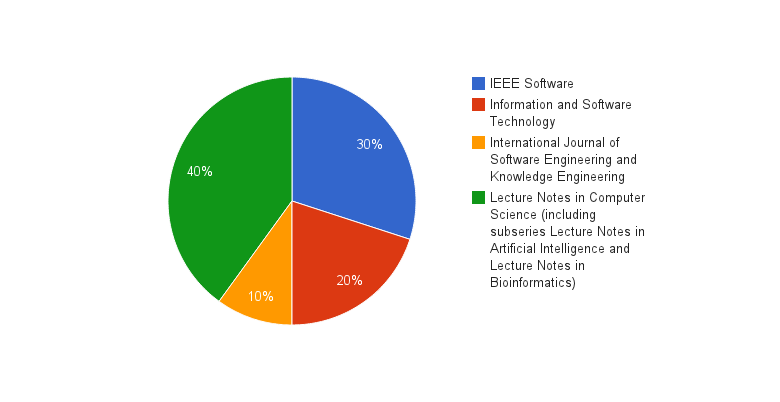
\includegraphics[width=200mm]{artikkelien_lehdet.png}
\caption{Lehdet, joissa valitut artikkelit on julkaistu.}
\label{artikkeli_lehdet_pie}
\end{figure}

Valituissa artikkeleissa on kuvattu jokin retrospektiivissä käytettävä menetelmä, joka sisältää juurisyyanalyysin käytön. Jotkin artikkeleista sisälsivät useamman menetelmän kuvauksen. Joissain tapauksissa toinen kuvattu menetelmä ei sisältänyt juurisyyanalyysiä \citep{staalhane2004root, dingsoyr2003extending}. Nämä menetelmät on jätetty huomioimatta tässä kandidaatintyössä.

Menetelmät on jaettu seuraaviin vaiheisiin: syötteen keräämiseen, kausaalianalyysiin ja parannusideoiden kehittämiseen. Vaiheiden sisältö eri menetelmien kohdalla on kuvattu taulukossa \ref{retrovaiheet_taulukko}. Menetelmien vaiheita on avattu tarkemmin pohdintakappaleessa.

\begin{center}
\begin{longtable}{|p{3cm}|p{4cm}|p{4cm}|p{4cm}|}
\caption{Artikkelien sisältämien retrospektiivimenetelmien vaiheet}\label{retrovaiheet_taulukko}\\ \hline
  & \textbf{Syötteen kehittäminen} & \textbf{Kausaalianalyysi} & \textbf{Parannusideoiden kehittäminen} \\
\hline
\endfirsthead
\multicolumn{4}{c}%
{\tablename\ \thetable\ -- \textit{Jatkoa edelliseltä sivulta}} \\
\hline
  & \textbf{Syötteen kehittäminen} & \textbf{Kausaalianalyysi} & \textbf{Parannusideoiden kehittäminen} \\
\hline
\endhead
\hline \multicolumn{4}{r}{\textit{Jatkuu seuraavalla sivulla}} \\
\endfoot
\hline
\endlastfoot
	\textbf{\citep{kalinowski2012evidence}} & Valitaan sopiva datajoukko, luokitellaan ja priorisoidaan se (Pareto-taulukko). & Syy-seurausdiagrammin, tarkemmin kalanruotodiagrammin, piirtäminen mainitaan hyväksi todetuksi tavaksi tunnistaa systemaattisten ongelmien syitä. & - \\ \hline
	\textbf{\citep{Lehtinen2011}} & Fokus-ryhmän tapaaminen, jossa kohdeongelma ja kausaalianalyysin osallistujat päätetään. & 1) Kerätään syitä anonyymisti sähköpostitse. 2) Muodostetaan kerätyistä syistä suunnattu verkko. 3) Brainwriting, brainstorming kokouksessa. Muodostetaan suunnattu verkko. 4) Tunnistetaan juurisyyt sähköpostikyselyn avulla. & Workshop, jossa parannusideoita kerätään brainwriting-menetelmällä yhdistettynä skeptiseen ja optimistiseen perspektiiviin. \\ \hline
	\textbf{\citep{Bjornson2009} menetelmä 1} & KJ-menetelmä & Kalanruotodiagrammi (ryhmäkeskustelu). & - \\ \hline
	\textbf{\citep{Bjornson2009} menetelmä 2} & KJ-menetelmä & Kausaalikartan muodostaminen KJ-menetelmän avulla. & - \\ \hline
	\textbf{\citep{karlsson2006case}} & Kerätään sopiva datajoukko, uudelleenarvioidaan se ja visualisoidaan saatu data. & 1) Keskustellaan visualisoidussa datassa ilmenevien ongelmien syistä. Fasilitaattori kirjoittaa keskustelusta muistiinpanoja. 2) Muistiinpanojen pohjalta luodaan taulukko, jonka avulla löydetään eri datapisteille yhteisiä kategorioita (juurisyitä). & Kehitysideoiden kerääminen ja priorisointi. \\ \hline
	\textbf{\citep{de2004learning}} & Kyselylomake 2) KJ-menetelmä / Semistrukturoitu haastattelu. & Kalanruotodiagrammi (ryhmäkeskustelu). & - \\ \hline
	\textbf{\citep{staalhane2004root}} & Pareto-analyysi defekteistä. & 1) Kalanruotodiagrammi (ryhmäkeskustelu) 2) Pisteytyksen avulla tunnistetaan olennaisimmat syyt (juurisyyt). & 1) Valituille syille kehitetään brainstorming-menetelmällä parannusideoita, jotka kootaan taulukkoon. Näistä äänestetään olennaisimmat, eli ne, jotka aiotaan toteuttaa. \\ \hline
	\textbf{\citep{staalhane2003post} menetelmä 1} & 1) Projektipäälliköltä taustatietoa projektista 2) KJ-menetelmä ja sen tulosten priorisointi. & Kalanruotodiagrammi & Osallistujat keksivät parannusideoita kalanruotodiagrammin perusteella. Tämän jälkeen kokous. Lopulta muodostetaan lista konkreettisista parannusideoista. \\ \hline
	\textbf{\citep{staalhane2003post} menetelmä 2} & 1) Dokumenteista projektin taustatietoja. 2) Strukturoitu haastattelu & Syy-seuraussuhteita tunnistetaan haastattelun aikana (fasilitaattorilla vastuu). & Osallistujat keksivät parannusideoita lukemansa retrospektiiviraportin perusteella. \\ \hline
	\textbf{\citep{dingsoyr2003extending}} & KJ-menetelmä & Kalanruotodiagrammi &  \\ \hline
	\textbf{\citep{birk2002postmortem}} & 1) Fasilitaattori tutustuu projektiin 2) Asetetaan tavoite 3) Datankeruu ja luokittelu (KJ-menetelmä,  semistrukturoitu haastattelu tai fasilitoitu ryhmäkeskustelu) 4) Datan priorisointi & Kalanruotodiagrammi (ryhmäkeskustelu) & - \\ \hline
	\textbf{\citep{card1998learning}} & 1) Valitaan sopiva datajoukko, luokitellaan ja priorisoidaan se (Pareto-taulukko). & Selvitetään ongelmien juurisyitä keskustelemalla ja tutkitaan löytyykö useampaan ongelmaan samoja syitä. Jos ongelman juurisyy ei löydy triviaalisti, käytetään kalanruotodiagrammia (ryhmäkeskusteluineen) apuna. & Fasilitoidun ryhmäkeskustelun avulla löydetään konkreettisia kehitysideoita. Näistä keskitytään niihin, joilla todennäköisimmin on merkittävä vaikutus ongelmiin. \\ \hline
\end{longtable}
\end{center}

\section{Pohdinta}
Tässä kappaleessa vastataan kandidaatintyön tutkimuskysymyksiin. Ensimmäiseen tutkimuskysymykseen vastataan kuvaamalla artikkelien retrospektiivimenetelmiä. Runkona tämän osion kuvauksille toimii taulukko \ref{retrovaiheet_taulukko}.

Vertailemalla menetelmiä ja niiden vaiheita keskenään pyritään löytämään niistä tehokkaimmat ja toimivimmat piirteet. 
Vertailun avulla ja menetelmän keveyttä arvioimalla ja sovittamalla sitä lyhytkestoiseen ja höyhenenkevyeen, ketterään retrospektiiviin vastataan toiseen tutkimuskysymykseen. Synteesi muodostetaan sille omistetussa kappaleessa. 

\subsection{Retrospektiivin eri nimitykset}
Vaikka retrospektiiveistä käytetään kirjallisuudessa lukuisia eri nimityksiä, niitä käsitellään tässä kandidaatintyössä samalla tavalla. Pohjimmiltaan retrospektiivi \citep{AgileRetros2006}, post-mortem analyysi \citep{staalhane2003post}, postmortem analyysi \citep{de2004learning}, postmortem review \citep{dingsoyr2003extending}, process review \citep{karlsson2006case}, project review \citep{karlsson2006case}, retrospective analysis \citep{karlsson2006case}, project retrospective \citep{karlsson2006case} ja retrospective review \citep{karlsson2006case} tarkoittavat samaa asiaa.

Retrospektiivi voi olla yleinen koko analysoitavan työrupeaman kattava tapahtuma tai sille voidaan antaa jokin tietty fokus \citep{staalhane2003post}. Fokusoituja retrospektiivejä ovat muun muassa Post-release Analysis of Requirements SElection Quality \citep{karlsson2006case} ja Defect Causal Analysis \citep{card1998learning} ja artikkelissa \citep{de2004learning} kuvattu Postmortem analyysi.

\subsection{Retrospektiivien vaiheet}
Se, että retrospektiivimenetelmien vaihejako on helppo muodostaa samankaltaiseksi, kuin juurisyyanalyysimenetelmien vaihejako \citep{Lehtinen2011} kiinnittää huomiota. Voidaan nähdä, että silloin, kun juurisyyanalyysiä käytetään osana retrospektiivin menetelmää, kyseinen menetelmä ei kokonaisuudessan eroa juurisyyanalyysin käytöstä muussa kontekstissa. Molemmat sisältävät samanlaiset vaiheet.

Retrospektiivi käsitteenä tarkoittaa vain katsomista taakse, eli jonkin menneen tapahtuman arviointia. Ketterät ohjelmistotuotantomenetelmätkään eivät määritä retrospektiivissä käytettävää menetelmää. Ne määrittelevät retrospektiivin tavoitteet, joita ovat yleensä konkreettiset tiimin työprosessin parannusehdotukset. Tavoitteena on välttyä toistamasta samoja ongelmia ja toistaa onnistumisia. On vaikea tehdä eroa juurisyyanalyysiä käyttävän retrospektiivin ja muussa yhteydessä prosessinkehitystä varten pidettävän ongelmanratkaisuun tähtäävän juurisyyanalyysin välille.

\subsubsection{Syötteen kehittäminen}
Syötteen kehittämisvaiheessa kerätään aiheita, jotka ovat olleet retrospektiivissä käsiteltävän työrupeaman (iteraatio, projekti) kannalta merkityksellisiä. Näistä aiheista valitaan tärkeimmät, joita analysoidaan tarkemmin seuraavassa kausaalianalyysivaiheessa. Artikkelien syötteen kehittämisvaihe voidaan jakaa varsinaiseen aiheiden keräämiseen, niiden ryhmittelyyn, sekä priorisointiin.

Kuudessa artikkelien kuvaamassa menetelmässä \citep{birk2002postmortem, dingsoyr2003extending, staalhane2003post, de2004learning, Bjornson2009} kahdestatoista käytetään syötteen kehittämisvaiheessa japanilaisen etnologin, Jiro Kawakita:n mukaan nimettyä fokusoitua brainstorming-menetelmää: KJ-menetelmää \citep{dingsoyr2003extending}. Jotkin artikkeleista suosittelevat KJ-menetelmää yhtenä vaihtoehtona muiden joukossa \citep{birk2002postmortem, staalhane2003post, de2004learning}. Artikkeleista \citep{birk2002postmortem} on ensimmäisenä suositellut KJ-menetelmää käytettäväksi retrospektiivin syötteen kehittämiseen.

KJ-menetelmässä jokainen osallistuja saa tietyn määrän post-it -lappuja. Jokainen kirjoittaa niille sovitun määrän hyviä ja huonoja kokemuksia analysoitavasta työrupeamasta. Jokainen esittää kirjoittamansa asiat ryhmälle ja asettaa laput valkotaululle. Osallistujat ryhmittelevät laput niiden aiheen mukaan ja keskustelevat niistä. \citep{birk2002postmortem}

Kaksi artikkelia kuvaa semistrukturoituja haastatteluja \citep{birk2002postmortem, de2004learning} ja yksi strukturoituja haastatteluja \citep{staalhane2003post}. Semistrukturoidussa haastattelussa fasilitaattori valmistelee listan kysymyksiä, jotka käsittelevät retrospektiivin aihetta \citep{birk2002postmortem}. Vaikkei tekniikkaa sen tarkemmin esitellä, vaikuttaisi siltä, että niiden avulla haastattelut pyritään ohjaamaan oikeaan suuntaan. Strukturoidussa haastattelussa suoritetaan kausaalianalyysi samalla, joten kysymyksillä pyritään ohjaamaan haastateltavat pohtimaan retrospektiivissä analysoitavan ongelman aiheuttajia \citep{staalhane2003post}.

Artikkelien \citep{kalinowski2012evidence, card1998learning} kuvaamassa Defect Causal Anlaysis -menetelmässä (DCA) valitaan virheraporttitietokannasta mahdollisimman kuvaava otos. Tämä osajoukko luokitellaan virhetyypin mukaan. Pääluokkien löytämiseen suositellaan Pareto-taulukon käyttämistä \citep{kalinowski2012evidence, card1998learning}. Pareto-taulukon avulla visualisoidaan ongelmien määrä ongelmatyypeittäin rymiteltynä \citep{card1998learning}.

Monissa artikkeleissa suositellaan kerätyn datan priorisointia \citep{card1998learning, birk2002postmortem, staalhane2003post, staalhane2004root, karlsson2006case}. Priorisoinnin avulla voidaan valita tärkeimmät aiheet, joita käsitellään kausaalianalyysivaiheessa. DCA-menetelmää kuvaavat artikkelit \citep{kalinowski2012evidence, card1998learning} käyttävät priorisoinnissa apuna Pareto-taulukkoa.

Artikkeli \citep{staalhane2004root} suosittelee Pareto-analyysin käyttämistä priorisointiin. Pareto-analyysi perustuu Pareto-periaatteeseen, jonka mukaan ilmiöissä usein noin 70 prosenttia seurauksista johtuu 30 prosentista syitä \citep{staalhane2004root}. 

Myös ryhmäkeskustelussa ilmenneiden prioriteettien perusteella voidaan muodostaa priorisoitu lista ongelmista \citep{staalhane2003post}. Artikkeli \citep{birk2002postmortem} ei ota kantaa siihen, miten priorisointi tapahtuu.

Artikkelissa \citep{Lehtinen2011} kuvatussa fokus-ryhmän tapaamisessa tehdään priorisointia, vaikkei sitä eksplisiittisesti mainitakaan. Kuvatussa fokus-ryhmän tapaamisessa valitaan yksi ongelma, joka otetaan käsiteltäväksi kausaalianalyysiin \citep{Lehtinen2011}.

\subsubsection{Kausaalianalyysi}
Kausaalianalyysivaiheessa tehdään varsinainen juurisyyanalyysi, eli analysoidaan, mistä valittu ongelma tai onnistuminen johtuu ja pyritään keksimään sille selittäviä syitä. 

Vaikka Ishikawan kalanruotodiagrammi \citep{ishikawa1990introduction} on kirjallisuudessa paljon käytetty syy-seuraussuhteiden visualisointitapa \citep{kalinowski2012evidence, Bjornson2009, de2004learning, staalhane2004root, dingsoyr2003extending, staalhane2003post, birk2002postmortem, card1998learning}, on kausaalinen kartta perustellusti osoitettu uudemmassa tutkimuksessa tehokkaammaksi visualisointitavaksi \citep{Bjornson2009, Lehtinen2011}. 

Kahdeksassa kymmenestä artikkelista kuvataan Ishikawa diagrammin (tunnetaan myös kalanruoto, eli fishbone-diagrammina) käyttöä kausaalianalyysissä \citep{kalinowski2012evidence, de2004learning, staalhane2004root, dingsoyr2003extending, birk2002postmortem, card1998learning}. Kahdessa artikkelissa kalanruotodiagrammi oli kuvattu toisena menetelmänä jonkin muun rinnalla \citep{Bjornson2009, staalhane2003post}. Kuvassa \ref{ishikawa_ex} on esimerkki kalanruotodiagrammista.

\begin{figure}[ht!]
\centering

\includegraphics[width=150mm]{ishikawa_esimerkki.png}
\caption{Esimerkki Ishikawan kalanruotodiagrammista}
\label{ishikawa_ex}
\end{figure}

Kalanruotodiagrammia käytetään syy-seuraussuhteiden visualisointiin. Ne piirretään yleensä kollaboratiivisesti retrospektiivin osallistujien kanssa etsittäessä syitä postiviivisille ja negatiivisille tapahtumille \citep{birk2002postmortem}. Valkotaululle kirjoitetaan analysoitavan tapahtuman nimi ja piirretään siihen osoittava suuri nuoli \citep{Bjornson2009}. Tapahtuman syyt visualisoidaan pienemmillä nuolilla, jotka osoittavat kohti suurta nuolta \citep{Bjornson2009}. Mahdolliset alisyyt piirretään pienempinä nuolina, jotka osoittavat kohti aiheuttamaansa seurausta \citep{Bjornson2009}. Näin muodostuu kalanruotoa muistuttava kuva \citep{birk2002postmortem}.

Bj{\o}rnson on tutkimuksessaan vertaillut Ishikawan kalanruotodiagrammin käyttöä kausaaliseen karttaan \citep{Bjornson2009}. On havaittu, että kalanruotodiagrammia ja ryhmäkeskustelua käytettäessä ryhmän aktiivisuus väheni verrattuna sitä edeltävään KJ-menetelmää hyödyntävään syötteen keräämisvaiheeseen \citep{Bjornson2009}, \citep{staalhane2003post}. Bj{\o}rnson kokeili KJ-menetelmää jokaista ryhmän jäsentä osallistavana toimintatapana myös juurisyyanalyysivaiheessa  ja sai rohkaisevia tuloksia sen toimivuudesta \citep{Bjornson2009}. Tähän tarkoitukseen hän tarvitsi kuitenkin kalanruotodiagrammia vapaamuotoisempaa diagrammityyppiä ja päätyi kausaalisen kartan käyttöön. Kuvassa \ref{verkko_ex} on esimerkki kausaalisesta kartasta.

\begin{figure}[ht!]
\centering
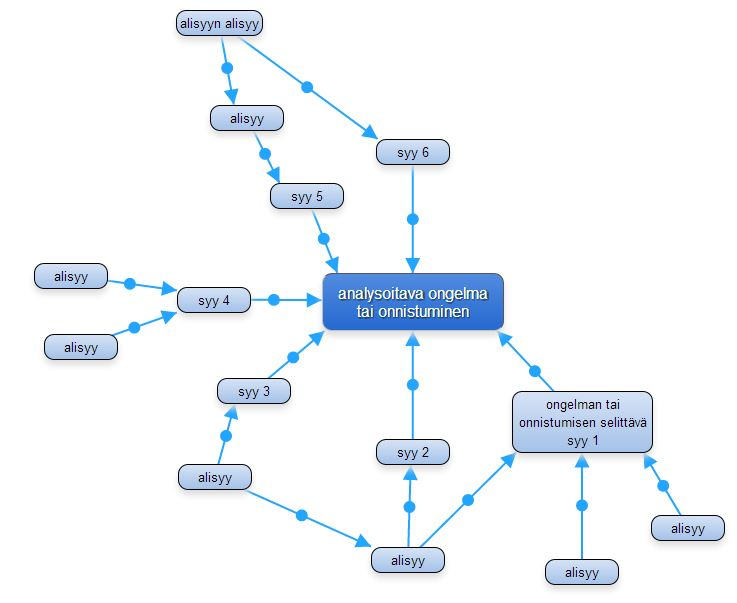
\includegraphics[width=150mm]{suunnattu_verkko_esimerkki_relaatioilla.jpg}
\caption{Esimerkki suunnatusta verkosta tai kausaalisesta kartasta (causal map)}
\label{verkko_ex}
\end{figure}

Myös Lehtinen käyttää ARCA-menetelmässään kausaalista karttaa, jota hän kutsuu suunnatuksi verkoksi \citep{Lehtinen2011}. Hän perustelee valintaa sillä, että toisin kuin kalanruotodiagrammissa, tai muissa syy-seuraussuhteiden esitystavoissa, suunnatussa verkossa samaa syytä ei tarvitse piirtää kuin kerran. Näin tehdään, vaikka se selittäisi useampaa muuta syytä samaan aikaan \citep{Lehtinen2011}. Muun muassa kalanruotodiagrammissa useamman syyn selittävät alisyyt pitää kopioida jokaiseen syyhyn erikseen \citep{Lehtinen2011}. 

Syyverkon Lehtinen muodostaa kahdessa eri vaiheessa: anonyymi syiden kerääminen ja kasuaalianalyysi-workshop. Anonyymissä syiden keräämisessä osallistujia pyydetään lähettämään sähköpostitse ainakin viisi syytä, jotka johtavat aiemmin valittuun kohdeongelmaan. Fasilitaattori muodostaa näistä omatoimisesti suunnatun verkon, jota täydennetään kausaalianalyysi-workshop:issa \citep{Lehtinen2011}. Workshop:issa Lehtinen käyttää Bj{\o}rnson:in tapaan KJ-menetelmän tyylistä osallistavaa lähestymistapaa syyverkon täydentämiseen.

Kausaalianalyyseistä vähiten systemaattisia lähestymistapoja kuvasivat artikkelit \citep{karlsson2006case} ja \citep{staalhane2003post}. Näissä menetelmissä syy-seuraussuhteita löydetään ryhmäkeskustelun aikana ilman, että niitä dokumentoidaan keskustelun aikana. Fasilittaattorin vastuulla on dokumentoida keskustelun aikana löytyneitä kausaalisuuksia.

Artikkelissa \citep{card1998learning} käytetään myös vapaamuotoisen tuntuista ryhmäkeskustelua tunnistamaan ongelmien juurisyitä. Kalanruotodiagrammi piirretään vain, jos onglmien juurisyyt eivät löydy triviaalisti. Tämäkään lähestymistapa ei vakuuta systemaattisuudellaan. Herää kysymys, minkälaisia artikkelissa kuvatut triviaalit tapaukset ovat. Miten toinen menetelmä voi pelkällä keskustelulla tunnistaa samoja olennaisia juurisyitä, mihin muut menetelmät tarvitsevat rakenteellisen, ja määritellyn menetelmän, sekä syy-seuraussuhteiden jatkuvan visualisoinnin analyysin tueksi.

Syy-seuraussuhteiden dokumentoinnin jälkeen ainoastaan artikkeleissa \citep{card1998learning, staalhane2004root, karlsson2006case, Lehtinen2011} valitaan kerättyjen syiden joukosta olennaisimmat juurisyyt, joihin aiotaan kehittää parannusideoita. Muissa artikkeleissa retrospektiivi loppuu syy-seuraussuhteiden dokumentointiin.

\subsubsection{Parannusideoiden kehittäminen}

Viisi artikkelien kuvaamaa retrospektiivimenetelmää kahdestatoista sisältää retrospektiivin päätteeksi pidettävän parannusideoiden kehittämisen \citep{card1998learning, staalhane2003post, staalhane2004root, karlsson2006case, Lehtinen2011}. Näistä artikkeleissa \citep{card1998learning, staalhane2004root, karlsson2006case, Lehtinen2011} kehitetään parannusideoita edellisessä vaiheessa valituille tärkeimmille juurisyille. Artikkelissa \citep{staalhane2003post} kausaalianalyysistä ei ole valittu tärkeimpiä juurisyitä, vaan parannusideoita kehitetään yleisesti syy-seuraussuhteiden visualisoinnin tai muun dokumentaation perusteella.

Parannusideoiden kehittämisessä voidaan käyttää apuna fasilitoitua ryhmäkeskustelua \citep{card1998learning, karlsson2006case}, brainstorming:ia \citep{staalhane2004root}, tai brainwriting:ia yhdistettynä skeptiseen ja optimistiseen perspektiiviin \citep{Lehtinen2011}. Näistä kaikki menetelmät käyttävät lopuksi priorisointia tärkeimpien parannusideoiden valitsemiseksi. 

Artikkeli \citep{staalhane2003post} luottaa parannusideoiden kehittämisessä väljempään lähestymistapaan. Siinä ensimmäisessä menetelmässä osallistujia pyydetään keksimään parannusideoita kalanruotodiagrammia tarkasteltaessa. Koko retrospektiiviä käsittelevän kokouksen jälkeen muodostuu lista konkreettisista parannusideoista. Toisessa menetelmässä osallistujat keksivät parannusideat retrospektiivistä kirjoitetun raportin perusteella. \citep{staalhane2003post}

Brainwriting toteutetaan siten, että jokainen osallistuja työstää vuorollaan yhdelle valitulle juurisyylle parannusideaa ja kirjoittaa sen paperille. Tietyn ajan jälkeen jokainen antaa paperinsa vierustoverilleen. Jokainen osallistuja osallistuu vuorollaan jokaisen juurisyyn parannusidean kehittämiseen. Paperit kierrätetään vielä kerran siten, että jokainen osallistuja pisteyttää kaikki kehitetyt parannusideat. Lopuksi eniten pisteitä saaneet ideat valitaan. \citep{Lehtinen2011}.

Esitetyistä parannusideoiden kehittämismenetelmistä systemaattisimmilta vaikuttavat brainstorming ja brainwriting. Fasilitoitu ryhmäkeskustelu tai artikkelin \citep{staalhane2003post} suosima epämääräinen ja suppeasti kuvattu menetelmä eivät vaikuta siltä, että niillä saataisiin parhaalla mahdollisella tavalla aktivoitua osallistujia. Niissä fasilitaattorin aktiivisuudella ja tyylillä lienee erityisen suuri vaikutus ryhmän osallistamisessa.

\subsubsection{Synteesi}
Vaikka kuusi artikkelin kuvaamaa menetelmää \citep{dingsoyr2003extending, staalhane2003post, de2004learning, Bjornson2009} kahdestatoista pohjautuu artikkelissa \citep{birk2002postmortem} kuvattuun retrospektiivi-menetelmään, on kandidaatintyön tekijän mielestä järkevää painottaa uudempaa tutkimusta, joka on osoitettu olevan tätä menetelmää tuloksellisempi. Uudemmalla tutkimuksella tarkoitetaan artikkeleja \citep{Lehtinen2011, Bjornson2009}, sillä vaikka \citep{kalinowski2012evidence} on artikkeleista tuorein, voidaan se mieltää mentelmän kuvauksen osalta ympäripyöreämmäksi versioksi aiemmasta DCA-menetelmää käsittelevästä artikkelista \citep{card1998learning}.

Osassa Bj{\o}rnsonin artikkelia vanhemmista artikkeleista käytetään epäsystemaattisen tuntuisia menetelmiä, kuten \citep{karlsson2006case, staalhane2003post} ja kausaalianalyysin osalta \citep{card1998learning}. Muissa artikkeleissa kuvatut menetelmät perustuvat artikkelin \citep{birk2002postmortem} kuvaamaan retrospektiivimenetelmään, josta Bj{\o}rnson esittää parannellun versionsa.

Kuitenkin on otettava huomioon, ettei yksikään artikkeleissa kuvatuista menetelmistä kuvaa suoraan ketterää retrospektiiviä, vaan suuremman mittakaavan retrospektiivejä, kuten projektin jälkeen pidettäviä reflektointeja. Artikkeleissa kuvatuista menetelmistä valitaan siis parhaat palat, minkä jälkeen niitä skaalataan kevyemmiksi ja siten paremmin sopiviksi ketterään retrospektiiviin.

Syötteen kehittämisvaiheeseen valitaan KJ-menetelmä, koska se on monissa artikkeleissa käytetty syötteen kehittämismenetelmä ja parantaa Bj{\o}rnsonin mukaan retrospektiivin osallistujien aktiivisuutta \citep{Bjornson2009}. KJ-menetelmän suorittamisen jälkeen priorioidaan positiivisiset ja negatiiviset kokemuksset ja valitaan niistä olennaisimmat.

Pareto-analyysi \citep{staalhane2004root}, Pareto-taulukko \citep{card1998learning, kalinowski2012evidence} tai brainwriting \citep{Lehtinen2011} olisivat kaikki hyviä, varmoja tapoja tehdä priorisointi oikein perustein. Ne ovat kaikki kuitenkin myös aikaa vieviä menetelmiä. Myös ryhmäkeskustelu \citep{staalhane2003post} voi viedä paljon aikaa. Perinteinen käsiäänestys voisi olla ketterän retrospektiivin tarpeisiin sopivan nopea ja tehokas tapa hoitaa priorisointi. Siinä käytäisiin ehdotetuista kokemuksista KJ-menetelmän suorituksen aikana ryhmitellyt kokemusluokat läpi. Jokainen saisi äänestää niistä yhtä suosikikseen. Eniten ääniä saanut kokemusluokka valittaisiin kausaalianalyysiin.

Synteesin kausaalianalyysiin valitaan menetelmäksi KJ-menetelmä ja syy-seuraussuhteiden visualisointiin suunnattu verkko, joita suositellaan artikkeleissa \citep{Lehtinen2011, Bjornson2009}. Kausaalianalyysin päätteeksi tärkeimmät juurisyyt valitaan käsiäänestyksellä. Höyhenenkevyen, ketterän retrospektiivin laajuuteen soveltuisi se, että juurisyitä valitaan vain pieni määrä, esimerkiksi yhdestä kolmeen kappaletta.

Parannusideoiden kehittämismenetelmien joukosta valitaan systemaattiselta ja kevyeltä vaikuttava, artikkelissa \citep{staalhane2004root} suositeltu menetelmä. Siinä parannusideat kehitetään osallistujien kesken brainstorming-tekniikalla, jonka tuloksena muodostetaan taulukko kehitysideoista. Niistä valitaan äänestämällä ne ehdotukset, jotka aiotaan toteuttaa \citep{staalhane2004root} seuraavan iteraation aikana. Äänestys voitaisiin suorittaa käsiäänestyksellä. Kehitystiimi voi valita parannusideoita toteutettavaksi sen verran, kuin se uskoo ehtivänsä toteuttaa seuraavan iteraation aikana. Kandidaatintyön tekijä arvioi oman kokemuksensa perusteella tämän olevan todennäköisesti noin 1-3 parannusideaa.

\subsection{Kandidaatintyön validiteetti}

Tässä kappaleessa pohditaan kandidaatintyön validiteettia ja sen uhkia käyttäen artikkelin \citep{runeson2009guidelines} määrittämää validointiskeemaa.

\subsubsection{Konstruktion validiteetti}
Konstruktion validiteetti kuvaa sitä, mitä uhkia tutkimusmenetelmät aiheuttavat tutkimuskysymyksien kannalta. Kandidaatintyön konstruktion validiteetti voidaan mieltää hyväksi. Systemaattinen kirjallisuuskatsaus on menetelmänä luotettava, tarkka ja toistettava. Tämä taataan sillä, että kaikki sen vaiheet on tarkkaan määriteltyjä ja dokumentoituja.

\subsubsection{Ulkoinen validiteetti}
Ulkoinen validiteetti kuvaa sitä, ovatko tutkimuksen tulokset yleistettävissä. Jos ne ovat, niin missä määrin?
Kandidaatintyön on tarkoitus kuvata sitä, minkälaisia menetelmiä kirjallisuus kuvaa juurisyyanalyysiä soveltaviin retrospektiiveihin. On mahdollista, ettei Scopus-tietokanta, johon aineistohaku tehtiin, sisällä kaikkia olennaisia artikkeleja. Scopus-tietokannan laajuudesta johtuen tämä on kuitenkin epätodennäköistä. Scopus-tietokanta sisältää yli 20 500 tieteellistä lehteä 5000 kustantajalta \citep{Scopus2013}.

Aineistohaku rajattiin ennalta karsittuun joukkoon, eli Scopus-tietokantaan. Sieltä valittiin pelkät tieteelliset artikkelit, jotka kaikesta kirjallisuudesta todennäköisimmin sisältävät objektiivista tutkimustietoa. Näistä valinnoista johtuen voidaan mieltää, että käytetty materiaali on ollut sisällöltään luotettavaa ja tasokasta.

Voi olla, ettei valittu hakutermimme saavuttanut kaikkia olennaisia artikkeleita, mikäli ne eivät sisältäneet termissä käytettyjä hakusanoja. Oletettavasti hakusanat kuitenkin kattavat suuren osan tavotelluista artikkeleista. Lisäksi hakutermin luotettavuutta lisää se, että hakutermi on muodostettu harkiten ja iteroiden. Lopullinen hakutermi muodostettiin yhdessä kandidaatintyön ohjaajan kanssa. 

Mainittujen perustelujen valossa voitaneen olettaa, että kandidaatintyön tulokset kattavat merkittävän osan niistä artikkeleista, jotka kuvaavat juurisyyanalyysiä soveltavia retrospektiivejä. Tulokset lienevät siis yleistettävissä juurisyyanalyysiä soveltavien retrospektiivien kuvaukseksi aiemmasta kirjallisuudesta.

\subsubsection{Luotettavuus}
Luotettavuus kuvaa sitä, kuinka paljon tulokset riippuvat tutkimuksen tekijästä. Voiko joku muu, joka toistaa samat tutkimuksen vaiheet odottaa saavansa samat tulokset?

Kandidaatintyön tulosten luotettavuutta uhkaa eniten se, että työn on suurimmalta osin suorittanut yksi henkilö (kandidaatintyön kirjoittaja) oman arviokykynsä mukaan. Kandidaatityön ohjaaja on auttanut kandidaatintyön tekijää esimerkiksi hakusanojen valinnassa ja lopullisen hakutermin muodostamisessa. Silti suorittava työ, kuten artikkelien arviointi ja rajaus on ollut kandidaatintyön tekijän vastuulla. On mahdollista, että joitain olennaisia artikkeleja karsiutui väärin perustein pois, mikäli kandiaatintyön tekijä oli tulkinnut työn tiivistelmää väärin.

Vaikka artikkeleista olisi rajattu väärin perustein muutama artikkeli, on perusteltua olettaa, että suoritettu systemaattinen kirjallisuuskatsaus kattoi huomattavasti laajemman joukon tieteellisesti merkittäviä artikkeleita, kuin ei-systemaattinen lähestymistapa. Ei-systemaattisessa lähestymistavassa kokeiltaisiin sattumanvaraisesti erilaisia hakusanoja eri hakukoneissa ja valittaisiin niiden hakutuloksista omien mieltymysten perusteella artikkeleita, konferenssipapereita ja muuta kirjallisuutta.

\section{Yhteenveto}
Tämän kandiaatintyön tavoitteena on vastata seuraaviin tutkimuskysymyksiin:
\begin{enumerate}
\item Minkälaisia menetelmiä aiemmassa kirjallisuudessa on esitetty juurisyyanalyysiä soveltaviin retrospektiiveihin?
\item Minkälainen juurisyyanalyysiä soveltava menetelmä voisi sopia ketterän ohjelmistokehitystiimin retrospektiiviin?
\end{enumerate}
Vastaus tutkimuskysymyksiin saatiin suorittamalla systemaattinen kirjallisuuskatsaus \citep{Kitchenham2007}. Kirjallisuuskatsauksessa käytiin läpi 108 Scopus-hakukoneella löydettyä tieteellistä artikkelia. Artikkeleista rajattiin pois ne, jotka eivät abstraktin, otsikon ja avainsanojen perusteella sisältäneet juurisyyanalyysiä soveltavaa retrospektiivimenetelmää.

Rajauksen jälkeen kandidaatintyön aineistoksi jäi kymmenen artikkelia, joiden kuvaamat retrospektiivimenetelmät ja niiden eri vaiheet kuvattiin ja analysoitiin. Retrospektiivin eri vaiheet sovitettiin kolmeen eri päävaiheeseen: syötteen keräämiseen, kausaalianalyysiin ja parannusideoiden kehittämiseen. 

Kahdestatoista artikkeleissa kuvatuista retrospektiivimenetelmistä kuusi perustuu artikkelissa \citep{birk2002postmortem} kuvattuun menetelmään, joka hyödyntää muun muassa KJ-menetelmää syötteen kehittämiseen ja Ishikawan kalanruotodiagrammia ja ryhmäkeskustelua kausaalianalyysiin. Vain viisi menetelmää sisälsi parannusideoiden kehittämisen. Uudempi tutkimus artikkeleissa \citep{Bjornson2009, Lehtinen2011} osoittaa KJ-menetelmän tyyppisen lähestymistavan yhdistettynä suunnattuun verkkoon toimivan kausaalianalyysissä artikkelissa \citep{birk2002postmortem} kuvattua menetelmää tehokkaammin.

Kandidaatintyön lopussa kuvatuista menetelmistä muodostettiin synteesi, jonka arvellaan soveltuvan ketterän retrospektiivin menetelmäksi. Synteesin syötteen kehittämisvaihe koostuu KJ-menetelmästä ja olennaisten asioiden valitsemisesta käsiäänestyksellä. Kausaalianalyysivaiheessa hyödynnetään KJ-menetelmää käyttäen suunnattua verkkoa visualisoimaan ongelman syy-seurausyhteydet. Tärkeimmät juurisyyt valitaan käsiäänestyksellä. Valituille juurisyille kehitetään parannusideoita käyttäen brainstorming-menetelmää, jonka tuloksena muodostetaan taulukko kehitysideoista. Kehitysideoista toteutettavat äänestetään käsiäänestyksellä.

Työn kannalta tulevaisuudessa kehitettäviä asioita ovat seuraavat. Kandidaatintyössä tehdyn systemaattisen kirjallisuuskatsauksen validiteettia voisi kasvattaa siten, että joku muu kuin kandidaatintyön tekijä toistaisi SLR:n tai ainakin osia siitä ja tarkistaisi tulisiko itse samaan tulokseen.

Tieteellisten artikkelien joukkoa, joka systemaattisen kirjallisuuksen puitteissa luetaan kokonaan, voisi myös kasvattaa. Näin artikkelien karsinta tapahtuisi varmemmin perustein, kuin vain abstraktin, otsikon ja avainsanojen perusteella tehty karsinta.

Lisäksi kandidaatintyön aloittamaa tutkimusta voisi jatkaa kokeilemalla kandidaatintyön synteesissä kuvattua menetelmää käytännössä, ohjelmistoyrityksen ketterän ohjelmistokehitystiimin iteraation päätteeksi pidettävässä retrospektiivissä. Tällä tavoin synteesin todellinen toimivuus voitaisiin todentaa oikeassa ympäristössä.